\chapter{Opis stworzonego rozwiązania}
\label{cha:rozwiazanie}

Niniejszy rozdział zawiera opis aplikacji, która została stworzona na potrzeby tej pracy. Krótki opis co zawieraja kolejne podrozdzialy/// TODO

%---------------------------------------------------------------------------
%---------------------------------------------------------------------------
\section{Założenia projektowe}
\label{sec:zalozeniaProjektowe}
Swtorzyć aplikację typu guper spełniającą wszystkie wymagania stawiane przez NFZ. Implementującą dokładnie algorytm grupera według wytycznych.
Określić model danych oraz zdefiniować algorytm.

Aplikacja zostanie napisana w języku JAVA jako aplikacja stand-alone z dostępem do swojej bazy wiedzy zapisanej w pliku. 
Użyty zostanie najnowszy framework do tworzenia GUI w JAVIE, najnowszy framework i metodologia Spring 3. Zastosowanie warstwowej architekury systemu.

Zaimplemnentowane zostanioe wszystko pod kątem systemu ekspertowego - tzn osobno baza wiedzy - osobno fakty - osobno reguły. Zaimplementowany zostanie własny mechanizm wnioskowania dostosowany do aktualnego rozwiązania.
Neiktóre warunki da sie zapisac w bazie danych. reguly mozna zaimplementowac w grovym - stworzyc interface. warunki kierunkowe - rowniez moga byc zapisane w bazie wiedzy - jako: nazwa - opis - skrypt groovy-iego.


%---------------------------------------------------------------------------
%---------------------------------------------------------------------------
\section{Architektura systemu}
\label{sec:architekturaSystemu}
kilka slow o architekturze systemu co to jest itp pierdu pierdu

%---------------------------------------------------------------------------
\subsection{Model 3-warstwowy}
\label{sec:model3warstwowy}
Architektura systemu odzwierciedla jego logiczny podział. Standardem w praktycznie każdej aplikacji jest zastosowanie architektury trójwarstwowej. Jest to bardzo stara idea i sięga roku 1978. Kiedy to komitet ANSI/SPARC wprowadził podział na trzy warstwy:
\begin{itemize}
 \item Fizyczną implementację systemu
 \item Abstrakcyjny model wycinka rzeczywistości odzwierceidlany przez system
 \item Sposób w jaki jest postrzegany z zewnatrz - spojrzenie z punktu widzenia użytkownika końcowego
\end{itemize}

Jeżeli odniesiemy architekurę trójwarstwową do systemów informatycznych to odpowiednikiem schematu wewnętrznego jest warstwa bazy danych, schematu konceptualnego - warstwa biznesowa, a schematu zewnętrznego warstwa aplikacji. Architekturę przedstawia rysunek:
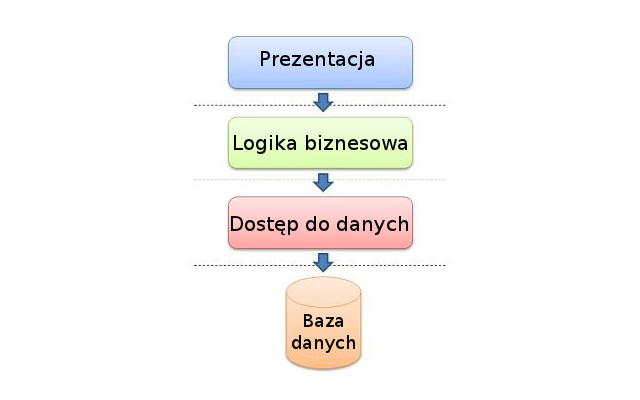
\includegraphics[scale=0.31]{images/3layer-architect}

Wybrałem ten model do zastosowania przy tworzeniu aplikacji ze względu na jego logiczną i zrozumiałą dla każdego informatyka modularność. Każda z warstw może zostać zaimplementowana w innym języku programowania, a łączą się one poprzez interfejsy. Dużym plusem tego rozwiązania jest łatwa możliwość zmiany pewnej części systemu bez zmian w innych częściach systemu. Dla przykładu, jeśli chcielibyśmy stworzyć GUI webowe to wystraczy tylko zaimplementować warstwę prezentacji i podpiąć się do warstwy logiki biznesowej.

%---------------------------------------------------------------------------
\subsection{Model architektury Spring}
\label{sec:modelArchitekturySpring}
Bardzo popularnym i nowoczesnym środowiskiem, które wprowadza zestaw narzędzi, wzorców oraz bibliotek potrzebnych do stworzenia nowoczesnych aplikacji serwerowych(i nie tylko) jest Springframework. Architektura Spring jest niesłusznie uważana za skomplikowaną, bardzo złożoną i niemożliwą do opanowania. W rzeczywistości architektura Spring stanowi zaawansowany przykład architektury szkieletowej umożliwiającej szybkie rozwijanie dowolnie złożonych aplikacji, niekoniecznie webowych. Konstrukcja szkieletu architektury Spring powoduje, że jest ona typem tzw. lekkiej infrastruktury, w której występuje bardzo niewielki stopień zależności od interfejsów Spring API. Architektura Spring obejmuje wszystkie warstwy aplikacji i podsuwa rozwiązania, które mogą być stosowane zarówno w warstwie prezentacji, jak i w warstwie integracji i warstwie danych. Architektura Spring jest rozwijana na licencji ,,open sourc'' od roku 2003 i od tego czasu zdobyła sobie dużą popularność i spore grono osób programujących. Poniższy rysunek ilustruje schemat architektury Spring:
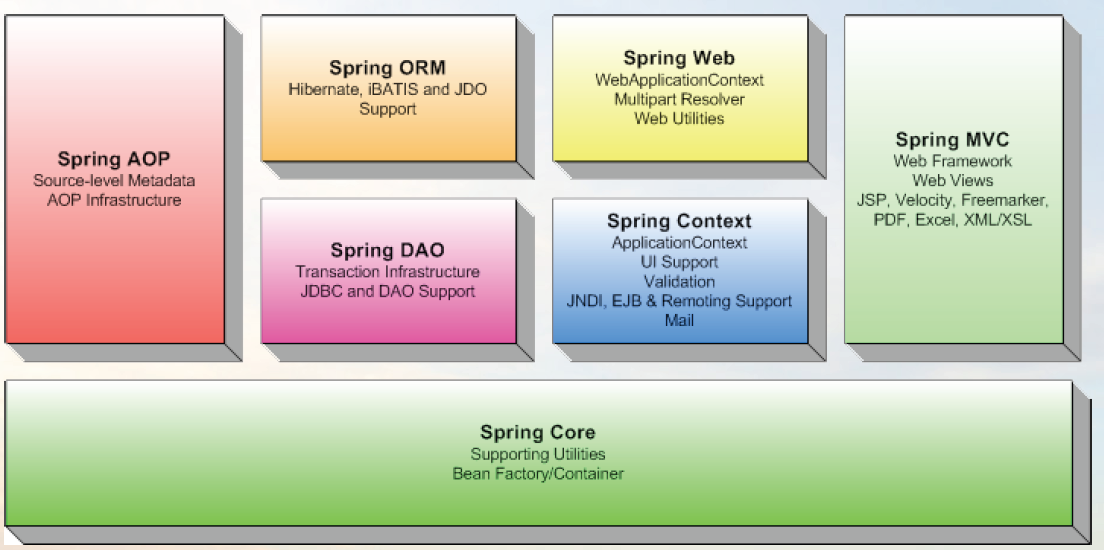
\includegraphics[scale=0.31]{images/spring-modules}
Architektura Spring składa się z kilku modułów, z których każdy może być wykorzystywany niezależnie w aplikacji. Oznacza to, że aplikacja może wykorzystywać całą moc architektury Spring, ale może także korzystać z fragmentu architektury, np. z modułu ułatwiającego dostęp do danych. Najważniejszym modułem architektury jest Spring Core, moduł oferujący zaawansowane opcje konfiguracji komponentów JavaBean oraz klas POJO(ang. Plain Old Java Object) i wykorzystujący technikę wstrzykiwania zależności.
Dla mojego rozwiązania postanowiłem skorzystać właśnie z tych dwóch fragmentów architektury Spring, tj dostęp do danych oraz Core dla warstwy serwisowej. Oto listing modułów Spring wykorzystywanych w projekcie:
\begin{itemize}
 \item JDBC - Java DataBase Connectivity - interfejs programowania opracowany w 1996 r. przez Sun Microsystems, umożliwiający niezależnym od platformy aplikacjom napisanym w języku Java porozumiewać się z bazami danych za pomocą języka SQL.
 \item DAO - Wzorzec projektowy Data Access Object (DAO) - rozdzielenie mechanizmu trwałości obiektów od reguł biznesowych
 \item Service - Spring Service Beans - obiekty serwisowe - wykonujące logikę biznesową
\end{itemize}

Dla warstwy prezentacji wykorzystałem również wsparcie Spring. W 2008 roku została wydana 1 wersja frameworku do tworzenia aplikacji desktopowych w JAVIE - SpringRCP - Rich Client Project. Niestety po wydaniu wersji 1.1 w 2009 projekt, który był na całkiem wysokim poziomie porównując do NetBeans-RCP lub Eclipse-RCP umarł śmiercią naturalną. W roku 2011 jeden z główynch projektantów Spring postanowił go odświeżyć. W niecałe 6 miesięcy przepisał cały framework używając najnowszej metodologii pochodzącej z Spring 3. Projekt ze względów politycznych musiał zmienić nazwę na Valkyrie-RCP. W kolejnych iteracjach dodanych zostało multum nowych funkcjonalności, w wyniku których po kolejnych 3 miesiącach powstało solidne narzedzie do tworzenia skomplikowanych aplikacji desktopowych w JAVIE. Jego podstawowe cechy to przejrzystość, prostota, stosowanie dobrych wzorców GUI. Kilka podstawowych elementów architektury Valkyrie:
\begin{itemize}
 \item Widget - komponent GUI (tabelka, forma, widok, edytor-danych)
 \item DataProvider - fasada danych dla komponentów UI.
\end{itemize}
Poniższy schemat przedstawia architekturę systemu jaki został zaimplementowany:
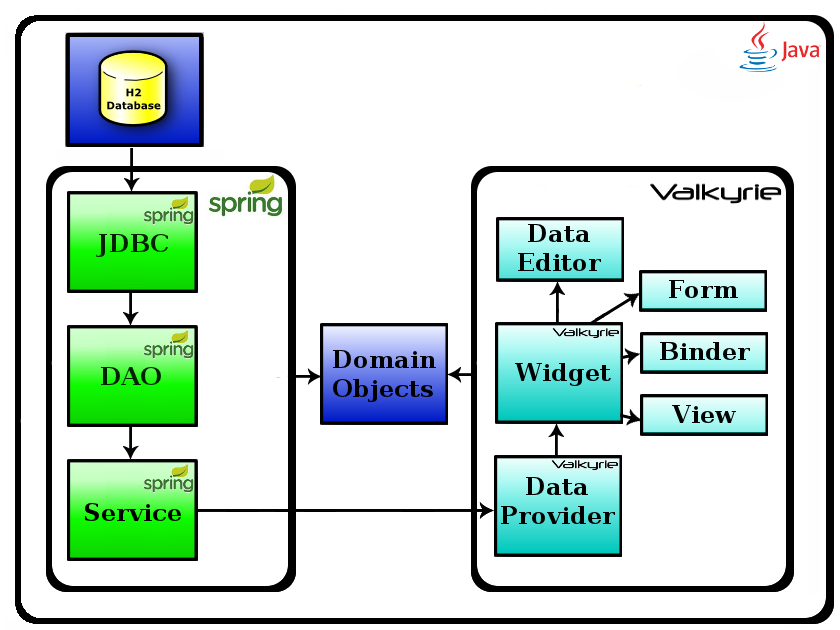
\includegraphics[scale=0.31]{images/spring-layers2}

Należy zaznaczyć, że model architektury spełnia założenia architekty trójwarstwowej:
\begin{table}[h]
 \caption{Moduły Spring jako elementy architektury trójwarstwowej}
 \small\tt
 \centering
 \vspace{0in}
 \begin{tabular}{|l|l|}
 \hline
 \textbf{3-warstwowa} & \textbf{Mój model} \\ 
 \hline
 Dostęp do danych & H2-Database, JDBC, DAO \\
 \hline
 Logika biznesowa & Services \\
 \hline
 Prezentacja & Valkyrie-RCP \\
 \hline
 \end{tabular}
\end{table}

%---------------------------------------------------------------------------
\subsection{Architektura systemu ekspertowego}
\label{sec:architekturaSystemuEkspertowego}
Jedna z definicji systemu ekspertowego definiuje go jako system charakteryzujący się strukturą:
\begin{itemize}
 \item Szkielet
       \begin{itemize}
	 \item Interfejs użytkownika
	 \item Edytor bazy wiedzy
	 \item Systemu wnioskujący
	 \item Mechanizm wyjaśniający
       \end{itemize}
 \item Baza wiedzy
 \item Danamiczna baza danych
\end{itemize}

Bardzo istotnym elementem systemu ekspertowego jest oddzielenie wiedzy dziedzinowej od reszty systemu. Takie podejście umożliwia usprawnienie działania systemu bez ingerencji w kod programu. W skrócie wyjaśnię elementy architektury systemu ekspertowego.

\textbf{Interfejs użytkownika} umożliwia zadawanie pytań, udzielanie informacji systemowi oraz odbieranie od systemu odpowiedzi i wyjaśnień.
\textbf{Edytor bazy wiedzy} pozwala na modyfikację wiedzy zawartej w systemie, umożliwiając tym samym jego rozbudowę.
\textbf{Mechanizm wnioskowania} jest głównym składnikiem systemu ekspertowego wykonującym cały proces rozumowania w trakcie rozwiązywania problemu postawionego przez użytkownika.
\textbf{Mechanizm wyjaśniający} jest to jeden z elementów interfejsu pomiędzy systemem a użytkownikiem, który umożliwia użytkownikowi uzyskanie odpowiedzi dlaczego system udzielił takiej, a nie innej odpowiedzi, albo dlaczego system zadał użytkownikowi określone pytanie.
\textbf{Baza wiedzy} jest to deklaratywna postać wiedzy ekspertów z danej dziedziny zapisana za pomocą wybranego sposobu reprezentacji wiedzy, najczęściej reguł.
\textbf{Danamiczna baza danych} jest pamięcią roboczą przechowującą pewne fakty wprowadzone w trakcie dialogu z użytkownikiem. Baza ta umożliwia odtworzenie sposobu wnioskowania systemu i przedstawienie go użytkownikowi za pomocą mechanizmu wyjaśniającego.
Architekturę systemu regułowego przedstawia poniższy schemat:
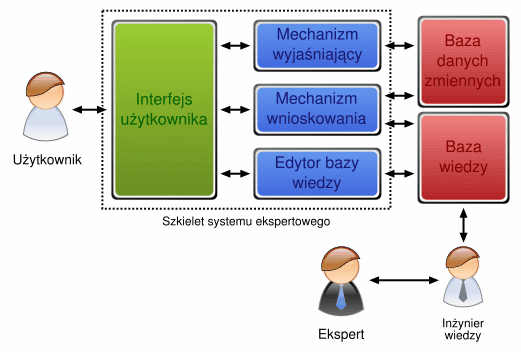
\includegraphics[scale=0.5]{images/expert-system}

%---------------------------------------------------------------------------
\subsection{System ekpertowy w architekturze Spring TODO ten podrozdzial poprawic na swiezo}
\label{sec:systemEkpertowyArchitekturaSpring}

Na pocztąku pracy postanwiona została teza: realizacja systemu ekspertowego w architekturze spring dla aplikacji grupera oraz jej optymalizacja.
Popularne narzędzia do implementacji systemu ekspertowego to język Prolog, lub system Drools. Bardzo przyjemne i co najważniejsze gotowe środowisko dla systemu ekspertowego. Jednak w mojej pracy postanowiłem zrobić coś innowacyjnego. Stworzyć przynajmniej zalążek silnika regułowego dla programu ekspertowego.
//TODO to zdanie poprawić: Dany problem może być rozwiązany w czystym języku JAVA, bo to nie język definiuje problem. Można napisać system typu klient-serwer w Prologu. Kwetsia jaki jest sposób postrzegania pewnych modułów i implementacja modułów jako developerów, żeby system był zalążkiem systemu ekspertowego.
A wieć zacząłem się zastanawiać co gdzie umieścić. Wynikiem jest projekt który element systemu mógłby być odpowiednikiem w architektruze innego systemu lub napisany przy pomocy tego modułu:
i tak:
---regułowy  ---   realizacja uzywajac elementow architektury spring
Baza wiedzy  ---  baza danych - dao - obiekty POJO odpowiedające regułom, skrypty groovy, sygnatury metod regułowych (ICondition, IRule)
dynamiczna baza dancyh - baza danych - dao - zwykłe obiekty POJO - moze interfejs oznaczajacy ze to jest fakt (IFact)

Interfejs uzytkownika - valkyrie-rcp springa - mozliwosc dodawania usuwania faktow, uruchamianie wnioskowania (wzorzec dataeditor - tabelka z filtrami i operacajmi CRUD)

Edytor bazy wiedzy - rowniez valkyrie-rcp springa - mozliwosc dodawania usuwania faktow (wzorzec dataeditor)(definiowanie faktow - roszerzenie)

Systemu wnioskujący - w warstwie biznesowej - service - uruchamiajacy mechanizm wnioskowania, wyciagajacy dla danych wejsciwoych(faktow) zestaw regul warunkow, uruchamiajacy sprawdzanie ich - wykonujacy dzialania jesli warunki jesli warunki sa spelnione. na wyjsciu podaje liste faktow spelniajacych warunki.

Mechanizm wyjaśniający - w warstwie biznesowej - sledzenie sciezki badania - zapisywanie na w danych wynikowych result - listy warunkow ktore zostaly sprawdzone.


%---------------------------------------------------------------------------
%---------------------------------------------------------------------------
\section{Model danych}
\label{sec:modelDanych}

W tym podrozdziale znajduje się opis w jaki sposób powstawał model danych dla aplikacji.

%---------------------------------------------------------------------------
\subsection{Dane wejściowe NFZ}
\label{sec:daneWejscioweNFZ}
Jedynym pewnym źródłem danych dla aplikacji były rozporządzenia NFZ. Fundusz opublikował ponad 30 wersji pliku parametryzującego, w formacie MS-Excel. W pliku parametryzującym znajdują się arkusze, w których zostały zapisane dane w postaci tabel zdefiniowanych przez NFZ. Każda następna wersja pliku parametruzyjącego przynosiła ze sobą zaktualizowane dane. Na przykład rozpoznania i procedury, które nie występowały w wersji wcześniejszej pliku parametryzującego. Z kolejnymi wydaniami wersji poprawiane zostały drobne błędy związane z formatem zapisu danych. Moją uwagę w trakcie porównywania wersji plików zwrócił zapis w kolumnie ranga procedury. Ranga większa niż 2 była zapisywana jako napis: '>2', co poprawiono na napis '3'. Ze względu na fakt, iż wiele poprawiono wraz z wydaniami kolejnych wersji pliku parametryzującego postanowiłem pracować na wersji 25, która jest jedną z najnowszych. 

Niestety nadal model danych pozostawiał wiele do życzenia. Na przykład w arkuszu o nazwie 'JPG' znajduje się listing wszystkich kodów JGP, jako kolumny przyjęte zostały wartości oddziałów - na przecięciu wiersza(kodu jgp, kodu produktu i nazwy jgp) i kolumny(oddział) postawiony został krzyżyk. W innym arkuszu dotyczącym wartości punktowej dla kodu JGP przepisane zostały jeszcze raz wszystkie kody jgp, kody produktu i nazwy jgp, a obok podane wartości punktowe. Kolejnym przykładem jest zdefiniowanie w arkuszu 'procedury' redundantnych danych - kody i nazwy procedur zduplikowane po 4-kroć, różniące się jedynie kolumną 'typ listy'.

Plik parametryzujący dostarczał redundantne dane, zduplikowane wartości w wielu tabelach, nieokreślone klucze podstawowe, obce, ograniczenia unikalności. Nasuwał się automatycznie jeden wniosek: model danych dostarczany przez NFZ musi koniecznie zostać przekonwertowany tak, aby nowy model danych zachowywał integralność. Konwersja bedzie polegała na zapimportowaniu danych z arkusza kalkulacyjnego do bazy danych, a następnie normalizacji bazy.

%---------------------------------------------------------------------------
\subsection{Relacyjna baza danych}
\label{sec:relacyjnaBazaDanych}

Postanowiłem wszystkie dane aplikacji przechowywać w relacyjnej bazie danych ze względu na nastepujące właściwości tego rozwiązania:
\begin{itemize}
 \item Wszystkie wartości danych oparte są na prostych typach danych.
 \item Wszystkie dane w bazie relacyjnej przedstawiane są w formie dwuwymiarowych tabel
 \item Po wprowadzeniu danych do bazy, możliwe jest porównywanie wartości z różnych kolumn, zazwyczaj również z różnych tabel, i scalanie wierszy, gdy pochodzące z nich wartości są zgodne. Umożliwia to wiązanie danych i wykonywanie stosunkowo złożonych operacji w granicach całej bazy danych.
 \item Wszystkie operacje wykonywane są w oparciu o algebrę relacji, bez względu na położenie wiersza tabeli.
 \item Z braku możliwości identyfikacji wiersza przez jego pozycję pojawia się potrzeba obecności jednej lub więcej kolumn niepowtarzalnych w granicach całej tabeli, pozwalających odnaleźć konkretny wiersz. Kolumny te określa się jako klucz podstawowy tabeli.
\end{itemize}
Uniwersalność tego rozwiązania pozwala zapisywać wszystkie typy danych, począwszy od typów prostych skończywszy na typach złożonych takich jak zserializowane obiekty JAVY, skrypty Groovy'iego lub pliki binarne. Według mnie takie podejście definiuje dużą elastyczność systemu. Na przykład planowana implementacja systemu ekspertowego będzie wymagała pewnego nakładu pracy projektowej i implementacyjnej szczególnie. Ale jestem przekonany, że rozwiązania tworzone pod konkretne problemy są lepiej zaprojektowane niż uniwersalne oraz najszybsze, co jest najważniejsze z punktu widzenia użytkownika końcowego.

Ważną decyzją jest również wybór silnika bazy danych. Ponieważ jednym z założeń projektowym było napisanie projektu w nowoczesnym języku programowania jakim jest JAVA postanowiłem wybrać silnik bazo-danowy napisany właśnie tylko i wyłącznie w czystej JAVIE. Szukałem również rozwiązania, które pozwoli mi na zapis/odczyt danych z pojedynczego pliku bez potrzeby instalacji całej machiny serwera w systemie operacyjnym. Skorzystałem z tabelki umieszczonej na stronie www.h2database.com:

\begin{table}[h]
 \caption{Porównanie właściwości}
 \tiny\tt
 \centering
 \vspace{0in}
 \begin{tabular}{|l|l|l|l|l|l|}
 \hline
  & \textbf{H2} & \textbf{Derby} & \textbf{HSQLDB} & \textbf{MySQL} & \textbf{PostgreSQL} \\
 \hline
 Pure Java & Yes & Yes & Yes & No & No \\
 \hline
 Memory Mode & Yes & Yes & Yes & No & No \\
 \hline
 Encrypted Database & Yes & Yes & Yes & No & No \\
 \hline
 ODBC Driver & Yes & No & No & Yes & Yes \\
 \hline
 Fulltext Search & Yes & No & No & Yes & Yes \\
 \hline
 Multi Version Concurrency & Yes & No & Yes & Yes & Yes \\
 \hline
 Footprint (jar/dll size) & ~1 MB & ~2 MB & ~1 MB & ~4 MB & ~6 MB \\
 \hline
 \end{tabular}
\end{table}

W końcu udało mi się znaleść silnik bazodanowy spełniający postawione przeze mnie wymagania. H2-database jest to rozwiązanie typu openSource, napisane w 100\% przez 1 osobę(Thomas'a Mueller'a). Zaletą silnika H2 jest jego innowacyjność. Autor stawia na łatwość użytkowania silnika bazy. Co objawia się bardzo łatwą konfiguracją, szybkim i prostym dostępem do administracji przez consolę H2, która jest uruchamiana w oknie przeglądarki. Funkcje importowania i eksportowania danych do/z plików zewnętrznych są wręcz intuicyjne. Dokumentacja do silnika jest przejrzysta spójna, cały czas na bieżąco aktualizowana. Chociaż rozwiązanie nie jest powszechnie znane, jednak tak duża firma jak Google stosuje go w niektórych swoich serwerowych rozwiązaniach.

%---------------------------------------------------------------------------
\subsection{Normalizacja danych}
\label{sec:normalizacjaDanych}

Dostarczony przez NFZ plik parametryzujący musi zostać poddany 'obróbce'. Każdy z arkuszy z pliku parametryzującego zapisałem w osobnym pliku CSV. Każdy z plików csv zaimportowalem(używając funkcji CSVREAD silnika H2) do osobnej tabeli tymczasowej.

\scriptsize
\begin{verbatim}
CREATE TEMPORARY TABLE ICD9_TMP(
    LIST_CODE_ID VARCHAR(5) NOT NULL, -- Kod listy
    LIST_TYPE_ID CHAR(1) NOT NULL,    -- Typ listy
    CODE VARCHAR(7) NOT NULL,         -- Kod procedury ICD-9
    RANGE INT,                        -- Ranga procedury ICD-9
    NAME VARCHAR(255) NOT NULL        -- Nazwa procedury ICD-9
) AS SELECT LIST_CODE_ID, LIST_TYPE_ID, CODE, RANGE, NAME FROM CSVREAD('icd9.csv');
\end{verbatim}
\normalsize

Po zaimportowaniu wszystkich tabel, następnym krokiem jest normalizacja bazy danych. Wprowadzenie kluczy publicznych i obcych, usunięcie zwielokrotnionych wierszy. Normalizaca według wykonywana była według 1PN, 2PN oraz 3PN. Kontynuując przykład z arkuszem 'icd9' napisałem skrypt SQL tworzący nowe tabele:

\scriptsize
\begin{verbatim}
CREATE TABLE ICD_LIST_TYPE(
    ID CHAR(1) PRIMARY KEY,
    NAME VARCHAR(10) NOT NULL
);

CREATE TABLE ICD9(
    CODE VARCHAR(7) PRIMARY KEY,
    RANGE INT,
    NAME VARCHAR(255) NOT NULL
);

CREATE TABLE ICD9_LIST(
    CODE VARCHAR(5) PRIMARY KEY
);

CREATE TABLE ICD9_LIST_CODE(
    ICD9_CODE VARCHAR(7) NOT NULL,
    LIST_CODE VARCHAR(5) NOT NULL,
    LIST_TYPE CHAR(1) NOT NULL,
    PRIMARY KEY (ICD9_CODE, LIST_CODE),
    FOREIGN KEY(ICD9_CODE) REFERENCES ICD9(CODE),
    FOREIGN KEY(LIST_TYPE) REFERENCES ICD_LIST_TYPE(ID),
    FOREIGN KEY(LIST_CODE) REFERENCES ICD9_LIST(CODE)
);
\end{verbatim}
\normalsize
Po utworzeniu poprawnego schematu danych importujemy dane z tabel tymczasowych:

\scriptsize
\begin{verbatim}
INSERT INTO ICD_LIST_TYPE (ID, NAME) VALUES ('G', 'globalna');
INSERT INTO ICD_LIST_TYPE (ID, NAME) VALUES ('U', 'do sekcji');
INSERT INTO ICD_LIST_TYPE (ID, NAME) VALUES ('H', 'do grupy');
INSERT INTO ICD_LIST_TYPE (ID, NAME) VALUES ('N', 'negatywna');

INSERT INTO ICD9 (CODE, RANGE, NAME)
 SELECT DISTINCT CODE, RANGE, NAME FROM ICD9_TMP ORDER BY CODE;

INSERT INTO ICD9_LIST (CODE)
 SELECT DISTINCT LIST_CODE_ID FROM ICD9_TMP ORDER BY LIST_CODE_ID;

INSERT INTO ICD9_LIST_CODE (ICD9_CODE, LIST_CODE, LIST_TYPE)
 SELECT CODE, LIST_CODE_ID, LIST_TYPE_ID FROM ICD9_TMP ORDER BY CODE;
\end{verbatim}
\normalsize

Postępując podobnie udało mi się przenieść wszystkie potrzebne dane z arkuszy kalkulacyjnych do tabel bazy danych SQL. Wprowadziłem relacje poprzez ustalenie kluczy publicznych oraz obcych. Dla kolumn wymagających wprowadzenia ograniczenia unikalności, zostało ono dodane. W miejscach gdzie spodziewałem się bardzo dużej ilości zapytań wyciągających dane po kolumnie wprowadziłem indeksację kolumny w celu szybszego działania instrukcji SELECT.
Wynikiem działania mojej pracy jest 16 plików SQL. Skrypty importują dane do tabel tymczasowych, następnie wykonują operacje tworzące tabele spełniając warunek spójności oraz zabiegające anomaliom bazo-danowym. Na samym końcu przepisujące dane. Skrypty zostały uporządkowane w kolejności, w której muszą zostać wykonane, aby stworzyć model bazy danych wypełniony danymi wejściowymi NFZ. Poniższy listing zawiera wszystkie wyróżnione tabele:

\begin{table}[h]
   \caption{Model danych}
   \tiny\tt
   \centering
   \vspace{0in}
   \begin{tabular}{|c|l|l|l|}
      \hline
      \textbf{arkusz} & \textbf{plik CSV} & \textbf{plik SQL} & \textbf{Nazwa tabeli} \\
      \hline
      wersja JGP & - & - & - \\
      \hline
      ograniczenie pobytu & - & 1\_time\_unit.sql & TIME\_UNIT \\
      \hline
      ograniczenie wieku & - & 2\_age\_limit.sql & AGE\_LIMIT \\
      \hline
      ograniczenie pobytu & - & 3\_hospital\_limit.sql & HOSPITAL\_LIMIT \\
      \hline
      JGP & jgp\_department.csv & 4\_department.sql & DEPARTMENT \\
      \hline
      ograniczenie trybu przyjęcia & - & 5\_income\_mode\_limit.sql & INCOME\_MODE\_LIMIT \\
      \hline
      ograniczenie trybu wypisu & - & 6\_outcome\_mode\_limit.sql & OUTCOME\_MODE\_LIMIT \\
      \hline
      - & - & 7\_patient.sql & PATIENT \\
      \hline
      wykaz specjalności komórek & specialization\_unit.csv & 8\_specialization\_unit.sql & SPECIALIZATION\_UNIT \\
      \hline
      wykaz specjalności komórek & specialization\_unit.csv & 8\_specialization\_unit.sql & SPECIALIZATION\_UNIT\_EXCLUDE\_SERVICE \\
      \hline
      listy procedur & icd9.csv & 9\_icd\_list\_type.sql & ICD\_LIST\_TYPE \\
      \hline
      listy procedur & icd9.csv & 10\_icd9.sql & ICD9 \\
      \hline
      listy procedur & icd9.csv & 10\_icd9.sql & ICD9\_LIST \\
      \hline
      listy procedur & icd9.csv & 10\_icd9.sql & ICD9\_LIST\_CODE \\
      \hline
      listy rozpoznań & icd10.csv & 11\_icd10.sql & ICD10 \\
      \hline
      listy rozpoznań & icd10.csv & 11\_icd10.sql & ICD10 \\
      \hline
      listy rozpoznań & icd10.csv & 11\_icd10.sql & ICD10\_LIST\_CODE \\
      \hline
      zakresy JGP & jgp.csv & 12\_jgp.sql & JGP \\
      \hline
      zakresy JGP & jgp.csv & 12\_jgp.sql & JGP\_POINT\_VALUE \\
      \hline
      mechanizm osobodni & jgp\_hospital.csv & 13\_jgp\_hospital.sql & JGP\_HOSPITAL \\
      \hline
      JGP & jgp\_department.csv & 14\_jgp\_department.sql & JGP\_DEPARTMENT \\
      \hline
      parametry JGP & jgp\_parameter.csv & 15\_jgp\_parameter.sql & JGP\_PARAMETER \\
      \hline
   \end{tabular}
\end{table}



%---------------------------------------------------------------------------
\subsection{Diagram ERD}
\label{sec:diagramERD}

W wyniku dogłębnej analizy oraz procesu projektowania bazy danych poprzez normalizację danych z pliku parametryzującego powstał spójny model danych. Logiczną strukturę wynikowego modelu ilustruje diagram ERD(Entity Relationship Diagram):

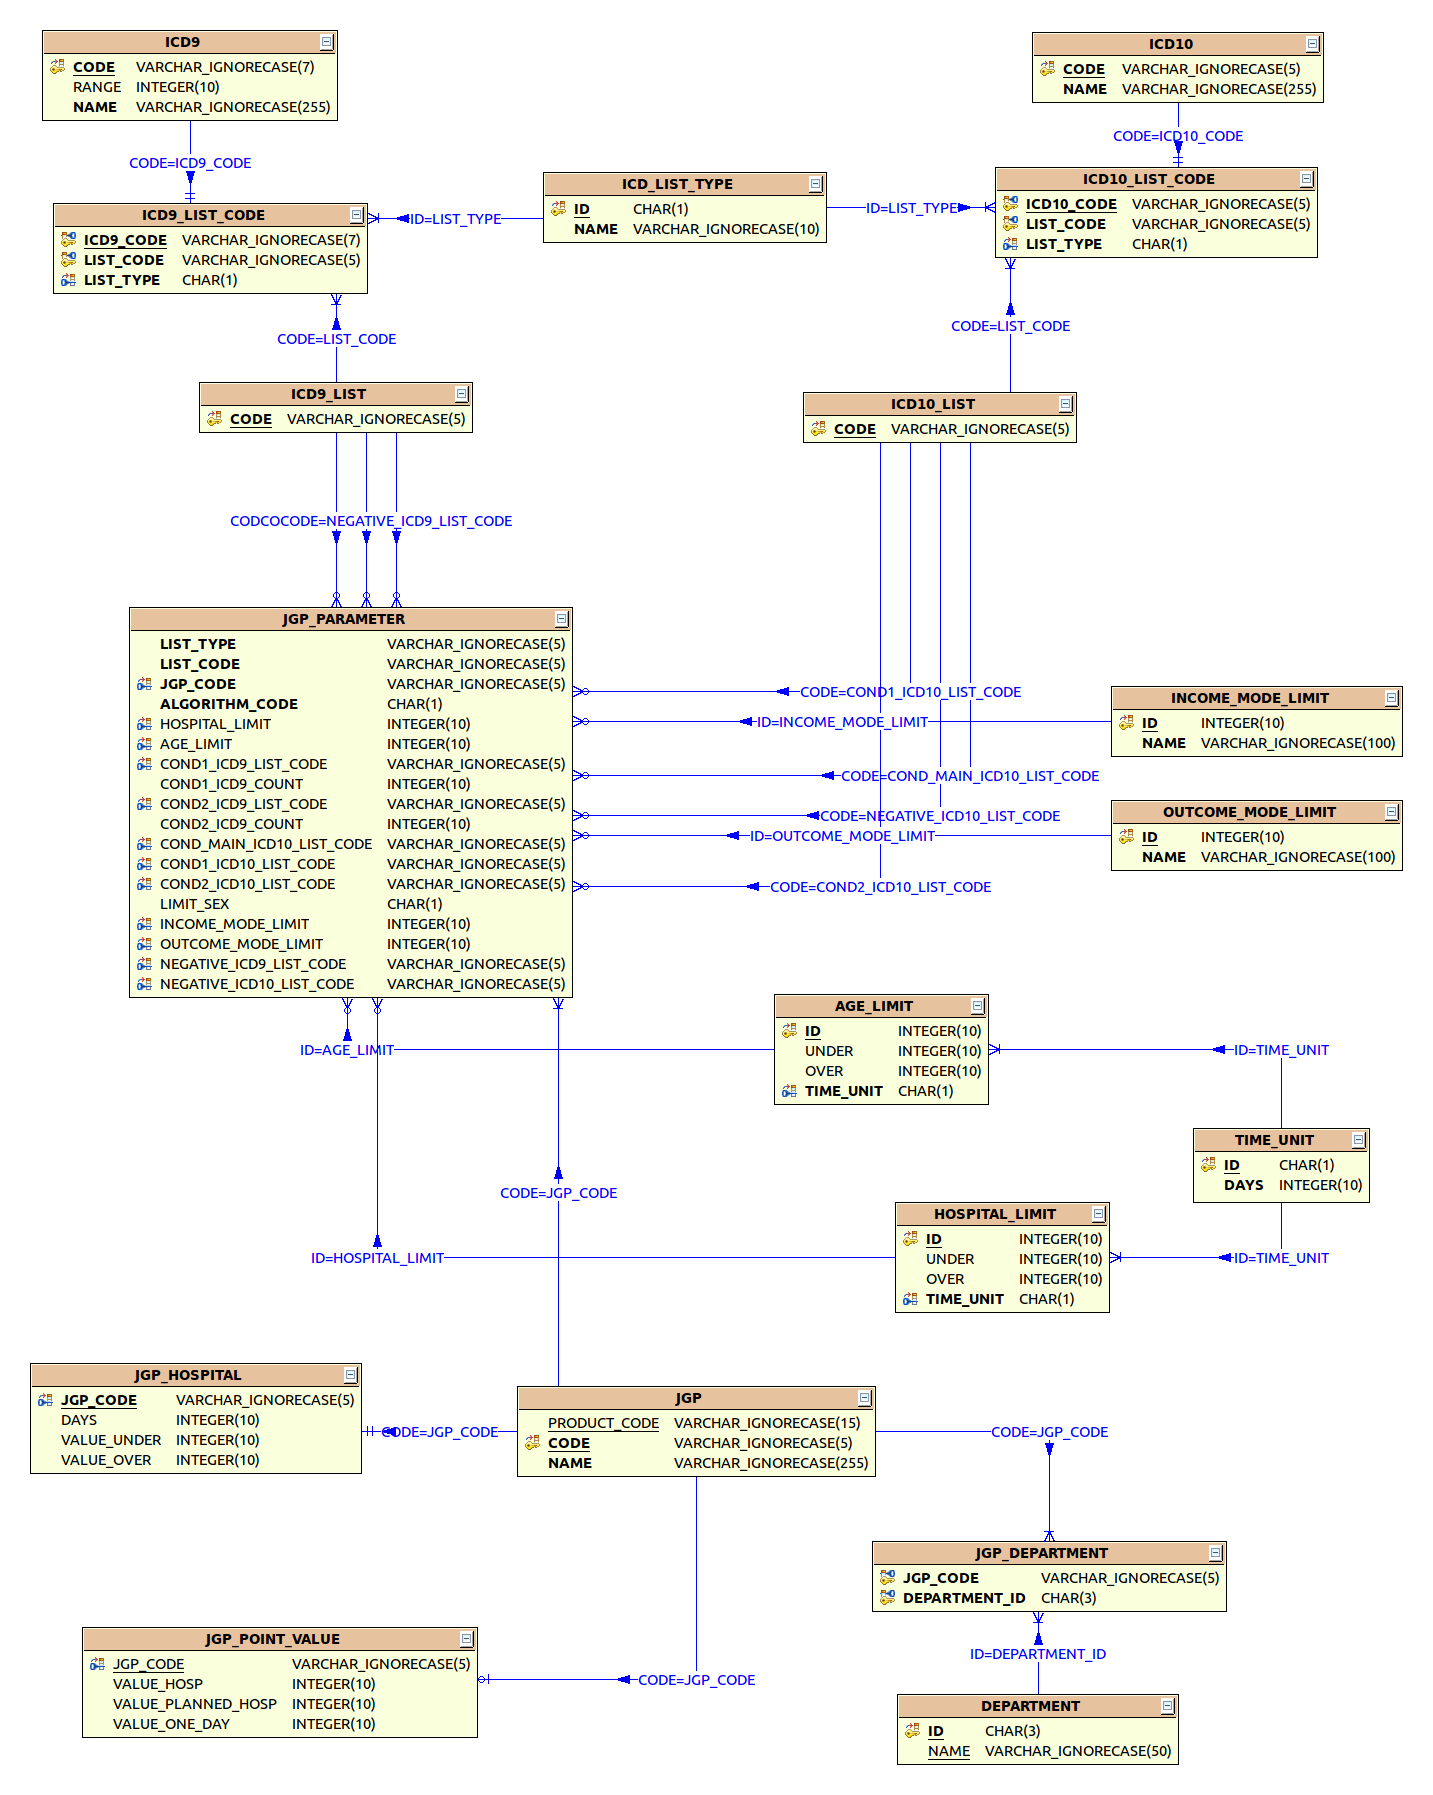
\includegraphics[scale=0.31]{images/erd}

%---------------------------------------------------------------------------
%---------------------------------------------------------------------------
\section{Gruper NFZ}
\label{sec:gruperNFZ}

W tym rozdziale znajduję się skrócony opis działania algorytmu grupera. Kompletny opis algorytmu grupera został przedstawiony w dokumencie upublikowanym przez NFZ zatytułowanym: "Informacje do przygotowania aplikacji grupera na potrzeby szpitalnych systemów informatycznych umożliwiającego kwalifikację rekordu pacjenta do właściwej grupy systemu Jednorodnych Grup Pacjentów". Dokument ten stał się podstawowym źródłem do stworzenia bazowej implementacji systemu. Dokument ten jest ponad 30-stronnicowym opisem, w jaki sposób powinna działać aplikacja gruper. Opis słowny algorytmu jak i schematy bloczkowe są dalekie do standardów takich jak język UML. Okazały się moim jedynym oraz kluczowym źródłem wiedzy o zasadach kierujących algorytmem. Rozpracowanie algorytmu grupera, poznananie i zrozumienie zasad jakimi się kieruje było kluczowym punktem mojej pracy.

%---------------------------------------------------------------------------
\subsection{Zasady i logika grupowania}
\label{sec:zasadyLogikaGrupowania}
Wynikiem działania algorytmu jest grupa JGP, która spełnia określony zestaw warunków. Zestaw grup JGP oraz warunków jest wyznaczany na podstawie danych wejściowych opisujących hospitalizację pacjetna. Alogorytm w uproszczeniu sprowadza się do wyznaczania grupy JGP. Po wyznaczeniu listy grup następuje badanie mechanizmem przeliczania, jeśli grupa kwalifikuje się do zmiany wartości zostaje ona zmieniona zgodnie z algorytmem mechanizmu przelcizania. Przedstawiony poniżej diagram aktywności przedstawia działanie algorytmu grupera:

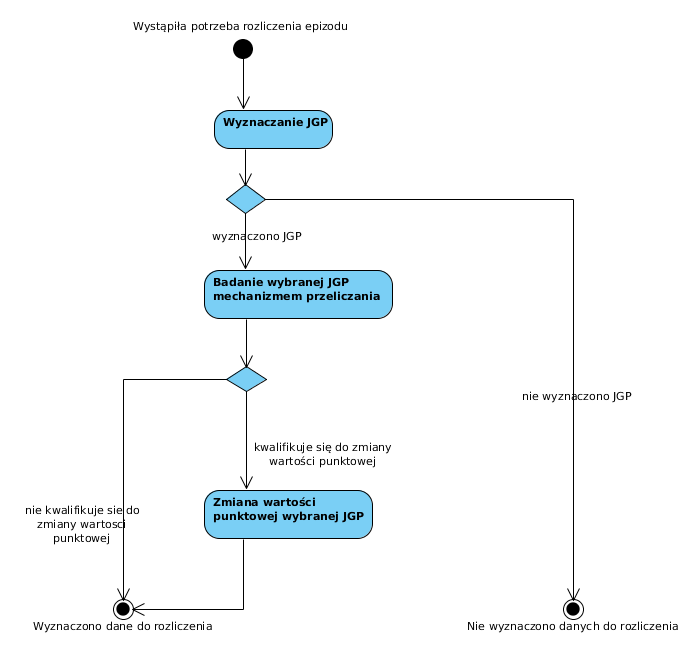
\includegraphics[scale=0.4]{images/activity-gruper}

%---------------------------------------------------------------------------
\subsection{Proces wyznaczania grupy systemu JGP}
\label{sec:procesWyznaczaniaGrupySystemuJGP}
Proces wyznaczania grupy można podzielić na dwie główne gałęzie. Pierwsza gałąź(tzw. ścieżka ICD-9) wyznacza zbiór zakwalifikowanych grup wraz z warunkami do sprawdzenia na podstawie procedur znaczących. Druga ścieżka 'ICD-10' wyznacza analogicznie zbiór zakwalifikowanych grup, ale na podstawie rozpoznań zasadniczych. Ścieżka dla rozpoznań jest wybierana przez program jeśli spełniony jest jeden z następujących warunków:
\begin{itemize}
\item w danych epizodu nie występuje żadna procedura
\item ranga procedury <= 2 i czas hospitalizacji > 1 dnia
\end{itemize}
Jeśli wymienione wyżej warunki nie są spełnione wybierana jest ścieżka ICD-9.

Następnie po wybraniu ścieżki wyznaczana jest lista kodów JGP wraz z warunkami do sprawdzenia. Każda grupa, która spełnia wszystkie warunki jest zapisywana na liście wybranych grup. Proces wyznaczania grupy dobrze ilustruje poniższy diagram aktywności:

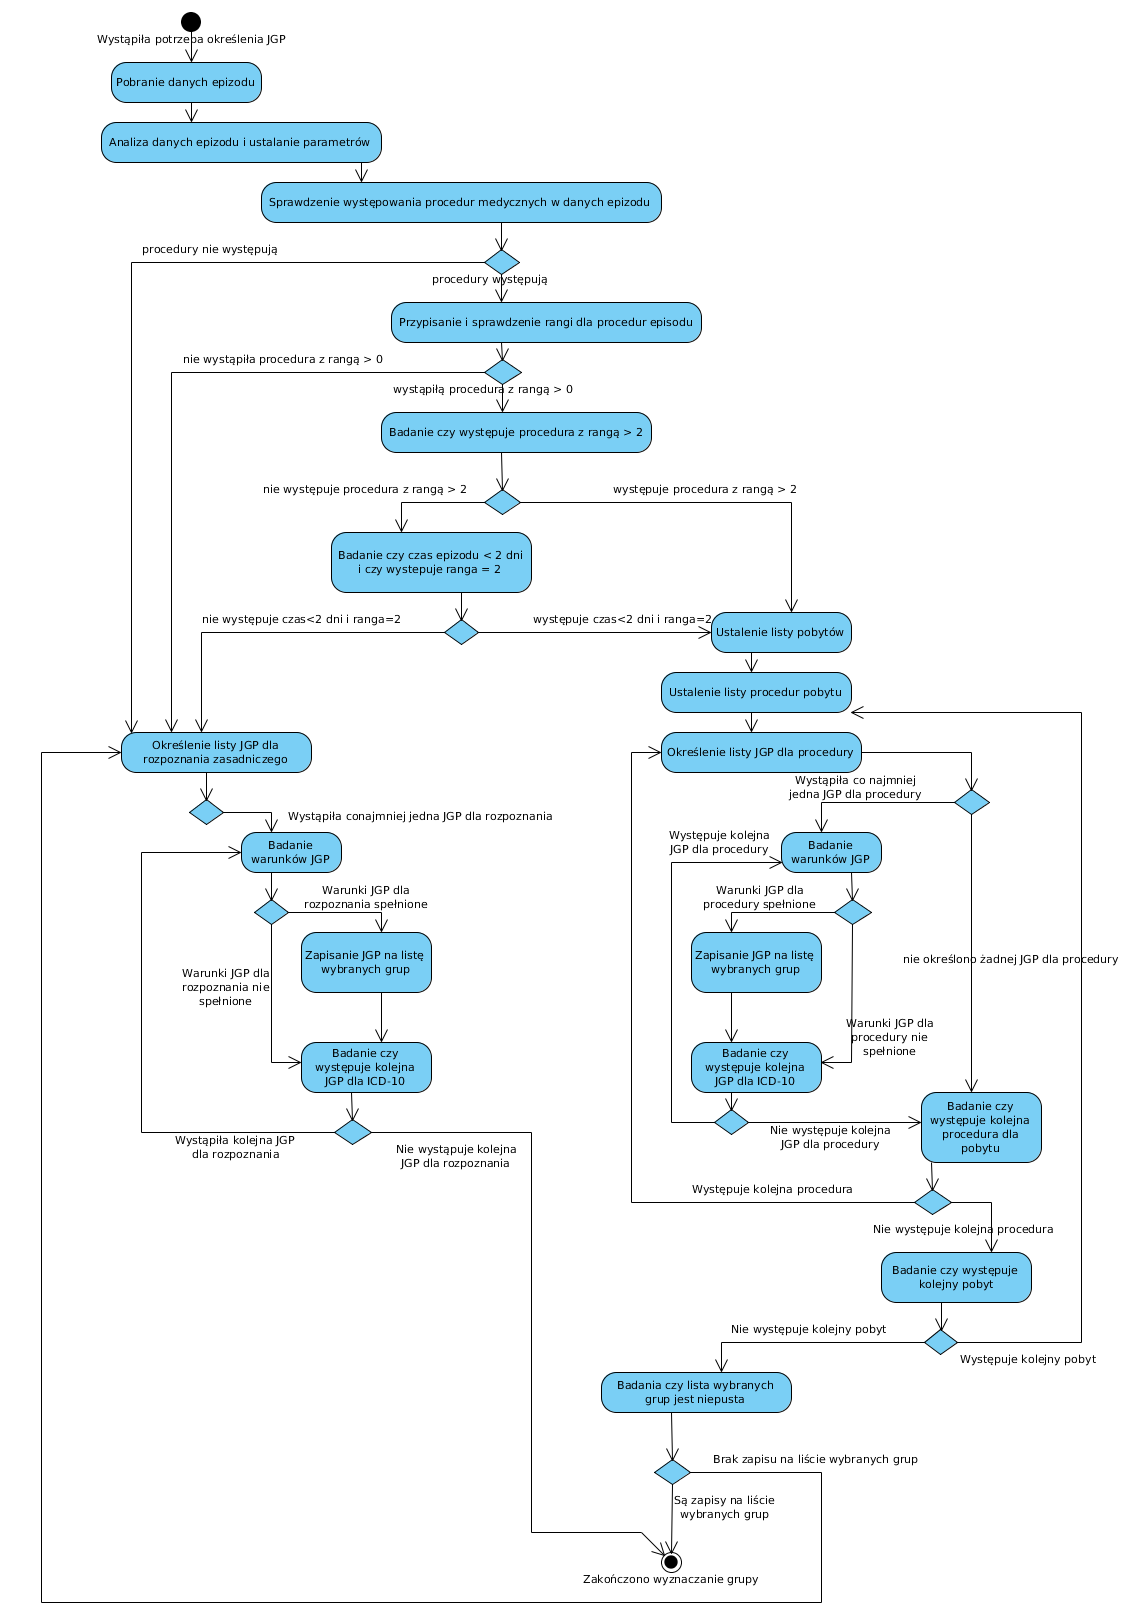
\includegraphics[scale=0.4]{images/activity-jgp} 

%---------------------------------------------------------------------------
\subsection{Warunki kierunkowe}
\label{sec:warunkiKierunkowe}
Warunki kierunkowe to decydujące o przebiegu grupowania ewentualne dodatkowe wymagania. Każdy z warunków został oznaczony literą alfabetu. A ich  dokładny opis znajduje się w dokumencie NFZ definiującym algorytm grupera. Procedura badająca warunki JGP w pierwszej kolejności sprawdza czy spełnione są warunki kierunkowe, ponieważ mają one decydujący wpływ na proces grupowania.
Sposób w jaki zdecydowałem się zaimplementować warunki kierunkowe:
\begin{itemize}
\item Każdy z warunków zapisany jest w bazie pojedynczą literą alfabetu (A-Z)
\item Dla obiektów domenowych literka alfabetu jest mapowana na odpowiednią wartość enuma Condition
\item zdefiniowanych jest 26 klas nazwanych dużymi literami alfabetu rozszerzających bazową klasę AbstractChecker oraz implementujących metodę:
  public abstract boolean checkCondition(Stay stay, JGPParameter parameter, List<Reason> reasons);
\item Utworzona została enum-mapa, w której kluczem jest enum(sygnatura warunku kierunkowego), a wartością obiekt(singleton) przypisanego do niej 'sprawdzacza' warunków
\end{itemize}
Zaletą tego podejścia jest możliwość implementacji w miarę uniwersalnego silnika do sprawdzania warunków kierunkowych. Działa on na zasadzie: dla każdego wybranego obiektu klasy JGPParameter(warunki które mają zostać sprawdzone) na podstawie odczytanej sygnatury warunku kierunkowego zostaje uruchamiany odpowiedni kawałek kodu JAVY sprawdzający warunki dla pobytu. A oto kawłek kodu realizujący tą funkcjonalność:
\scriptsize
\begin{verbatim}
private boolean checkDirectional(Stay stay, JGPParameter parameter, List<Reason> reasons) {
  //pobranie sygnatury(A-Z) warunku który powinien zostać sprawdzony
  Condition condition = parameter.getCondition();
  //pobranie checkera dla warunku z mapy
  AbstractChecker checker = conditionsMap.get(condition);
  Assert.notNull(checker, "not implemented checker for condition: " + condition);
  //uruchomienie odpowiedniego checkera i zwrócenie wyniku badania warunku
  return checker.checkCondition(stay, parameter, reasons);
}
\end{verbatim}
\normalsize
W ten sposób udało mi się zapisać bardziej skomplikowane warunki w bazie danych. Tak naprawdę zapisana jest sygnatura checkera, a niestety dalej ważna część logiki jest zapisana w kodzie. Ale o rozszerzeniu tego rozwiązania  i zapisaniu całej logiki checkera do bazy danych napiszę więcej w rozdziale system ekspertowy.

%---------------------------------------------------------------------------
\subsection{Mechanizm osobodni}
\label{sec:mechanizmOsobodni}
Oczywistym faktem jest, że wyznacznikiem kosztów leczenia pacjenta nie może być tylko wartość wyliczona na podstawie przypisanej do pacjenta grupy systemu JGP. Ważnym czynnikiem generującym koszty leczenia jest czas pobytu w szpitalu(pożywienie, wymiana pościeli, podawane leki) wszystkie te koszty generowane są przez pacjenta w każdym dniu. Dlatego do algorytmu grupera wprowadzony został mechanizm osobodni. Przelicza on wyznaczoną wartość punktową w przypadku spełnienia pewnych warunków dla określonej grupy według określonych zasad. Na początku algorytm bada czy można zastosować mechanizm przeliczania:
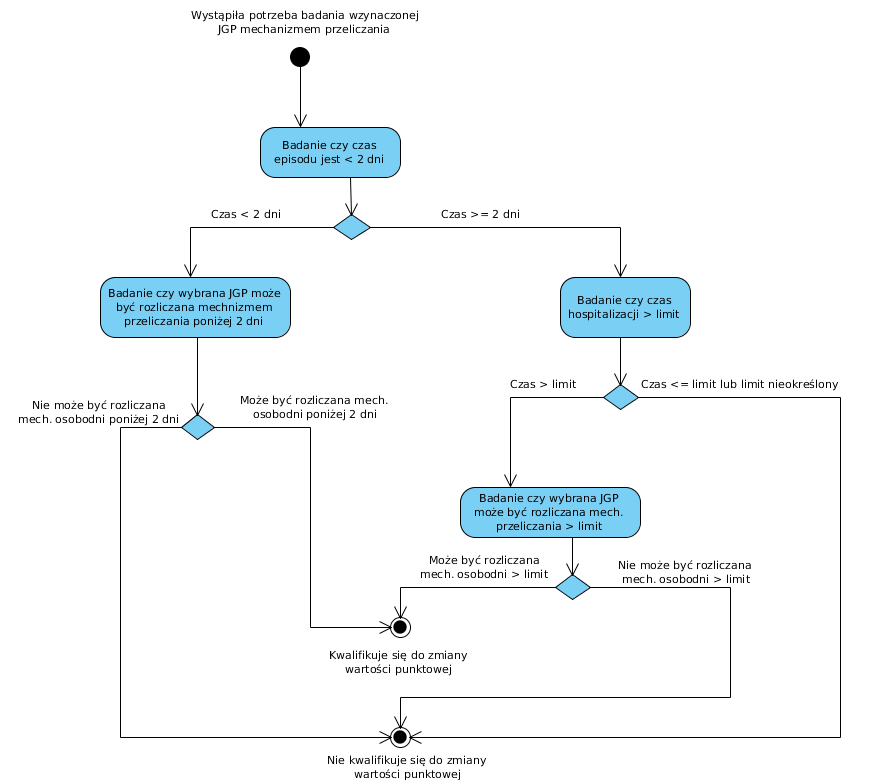
\includegraphics[scale=0.5]{images/activity-manday}

Jeśli wyznaczona grupa JGP dla epizodu nie kwalifikuje się do zmiany punktowej, pozostawiamy wartość wyznaczoną przez algorytm wyznaczania JGP. Natomiast jeśli zachodzi potrzeba zmiany punktowej stosujemy następujący algorytm dla 2 przypadków:
\begin{itemize}
\item Jeśli czas hospitalizacji jest mniejszy od 2 dni ustalamy nową wartość punktową ustalaną na podstawie wartości 'poniżej 2 dni' z obiektu klasy JGPHospital. Należy zaznaczyć, że z powyższego mechanizmu są wyłączone zgony, świadczenia rozliczane w ramach umów z zakresu ,,zespół opieki dziennej'' oraz ,,zespół chirurgii jednego dnia''.
\item Jeśli czas trwania episodu jest większy lub równy 2 dni i jest większy od limitu ustalonego na podstawie wartości ,,dni'' z obiektu klasy JGPHospital. To wartość JGP jest ustalana poprzez powiększenie aktualnej wartości JGP o wynik iloczynu dni powyżej limitu z wartością punktową określoną przez wartość "powyżej".

NOWA WARTOŚĆ PUNKTOWA = STARA WARTOŚĆ + RÓŻNICA DNI PONAD LIMIT * WAROŚĆ Z KOLUMNY POWYŻEJ
\end{itemize} 

%---------------------------------------------------------------------------
%---------------------------------------------------------------------------
\section{System ekspertowy}
\label{sec:systemEkspertowy}

\subsection{Klasyfikacja}
\label{sec:klasyfikacjaSystemuEkspertowego}
W tym podrozdziale chcę zakwalifikować system ekspertowy do odpowiednich klas systemów ekspertowych:
\begin{itemize}
 \item Ze względu na możliwość ingerencji człowieka w produkowane przez system rozwiązanie jest to tzw. system doradczy \textendash{} podpowiada rozwiązanie pomagając podjąć decyzję użytkownikowi \textendash{} prezentuje rozwiązanie jakiegoś problemu, ale do użytkownika należy jego ocena, oraz to czy je zaakceptuje, czy odrzuci.
 \item Ze względu na złożoność jest to system płytki - tzn. taki który korzysta tylko z informacji zgromadzonych w bazie wiedzy.
 \item Ze względu na dane otrzymywane na wyjściu jest to system:
   \begin{itemize}
    \item Diagnozy \textendash{} ocena istniejącego stanu na podstawie posiadanych danych
    \item Planowania \textendash{} opis stanu, do którego należy dążyć
   \end{itemize}
 \item Ze względu na rodzaj przetwarzanej informacji jest to system z wiedzą pewną.
\end{itemize}

\subsection{Baza wiedzy}
\label{sec:bazaWiedzy}
Najważniejszym z punktu widzenia systemu ekspertowego jest podział wiedzy na bazę faktów oraz bazę reguł. Logiczne wyróżnienie faktów dla systemu grupera JGP, pozwoli spojrzeć na system grupera jak na system ekpertowy. Wyróżnijmy więc fakty:
\begin{itemize}
 \item Rekord pacjenta
 \item Płeć
 \item Oddział
 \item Rozpoznanie(ICD-10)
 \item Procedura(ICD-9)
 \item Tryb przyjęcia
 \item Tryb wypisu
 \item Jednorodna Grupa Pacjentów
 \item Wartości punktowe dla JGP
 \item Czas hospitalizacji
\end{itemize}

oraz reguły:
\begin{itemize}
 \item warunki kierunkowe
 \item warunek na rozpoznanie główne
 \item warunek na rozpoznanie dodatkowe
 \item warunke na procedurę zasadniczą
 \item warunki na procedury dodakowe
 \item warunek na procedury i rozpoznania wykluczające się	
 \item ograniczenie na czas hospitalizacji
 \item ograniczenie na wiek
\end{itemize}
Spełnienie wyżej wymienionych warunków powoduje wykonanie akcji: zapisanie kodu JGP na listę kodów zaakceptowanych przez system. Model ten stosowany jest do wyznaczania grupy JGP.
Podobny mechanizm działa w trakcie wyznacznia nowych wartości mechanizmem osobodni.
Sprawdzane są warunki na czas hospitalizacji i jeśli są one spełnione wyznaczana jest nowa wartość punktowa.

\subsection{Maszyna wnioskująca}
\label{sec:maszynaWnioskujaca}
Realizacja maszyny wnioskującej w języku JAVA odbywa się przy użyciu Spring 3 na poziomie warstwy biznesowej. Klasa serwisowa przeprowadzająca proces wnioskowania zgodnie z wymaganiami systemu JGP to JGPService:
\begin{verbatim}
public interface JGPService {

    public List<JGP> findJGP(final JGPFilter filter);

    public JGPGroupResult group(Episode episode);

    public JGPGroupResult doByProcedures(Episode episode);

    public JGPGroupResult doByRecognitions(Episode episode);

    public void resolveResultsByJGP(Stay stay, List<JGPParameter> parameters, JGPGroupResult jgpGroupResult);

    public void recountManDay(Episode episode, List<JGPResult> jgpResultList);
}
\end{verbatim}

Metoda ,,group'' sprawdza którą ścieżkę wnioskowania obiera system - 2 opcje: wg. rozpoznania głównego lub wg. procedur zasadniczych. Metody ,,doByRecognitions'' oraz ,,doByProcedures'' wyznaczają zbiór warunków z charakterystyki JGP do przeanalizowania. metoda ,,resolveResultsByJGP'' wykonuje zasadnicze wnioskowanie:
\begin{itemize}
\item Sprawdza warunki określone w obiekcie parameters i jeśli zostaną zaakceptowane zapisuje je na liście accepted.
% \item Warunki niespełnione(wraz z powodami niezaakceptowania!) zapisuje na liście notAccepted, tworząc w ten spsób alternatywny sposób dojścia do lepszego rozwiązania.
\item Metoda sprawdza warunki kierunkowe, warunek na płeć, warunek na tryb przyjęcia i wypisu, warunek na leczenie w danym oddziale, warunki na współisteniejące i zasadnicze kody ICD , warunki na kody ICD wykluczające się(negatywne).
\end{itemize}

Podusmowując maszyna wnioskująca dla poszukiwania optymalnej grupy JGP realizuje proces wnioskowania w następujących krokach. Przyjmuje zbiór faktów wejściowych w postaci obiektu klasy Episode. Następnie wybiera ścieżkę według, której mają zostać ustalone parametry JGP(ICD9 lub ICD10). Po ustaleniu ścieżki - wyciągane są z bazy reguły które mają zostać sprawdzone w postaci obiektu klasy JGPParameter. Następuje sprawdzenie warunków i w przypadku spełnienia wszystkich grupa zostaje zapisana na liście zaakceptowanych grup.


%---------------------------------------------------------------------------
%---------------------------------------------------------------------------
\section{Optymalizacja JGP}
\label{sec:optymalizacjaJGP}

W tym podrozdziale opisane zostanie zagadanienie optymalizacji kosztów leczenia pacjenta. W poprzednim podrozdziale ustaliliśmy, że maszyna wnioskująca wybiera zbiór parametrów do przetestowania. Następnie dla grup JGP spełniających warunki zapisuje je na liście ,,zaakceptowane''. W tym miejscu nasunęła się pewna myśl: A może by tak spróbować zapisać grupy JGP, które były testowane a odrzucone przez algorytm na listę grup niezaakceptowanych? Może dla każdej niezaakceptowanej grupy JGP obliczyć jaką wartość punktową mogłaby przyjąć gdyby była zaliczona. Oraz usprawnienie/ idea: dla każdej niezaakceptwanej grupy zapisać na liście powód -> dlaczego została ona niezaakceptowana - jakich warunków nie spełniła?

REALIZACJA: Aby zrealizować założenia, należało rozwinąć istniejący algorytm. Do obiektu klasy JGPResult dodałem listę niezaakceptowanych grup. Każda niezaakceptwana grupa będzie posiadać dodatkowo listę powodów niezaakceptowania - lista obiektów klasy Reason. W ten sposób, system będzie wiedział jakie warunki były testowane dla konkretnego rozwiązania oraz dlaczego nie zostały one zaakceptowane. 
Stworzyłem hierarchię klas dla powodów niezaakcpetowania:

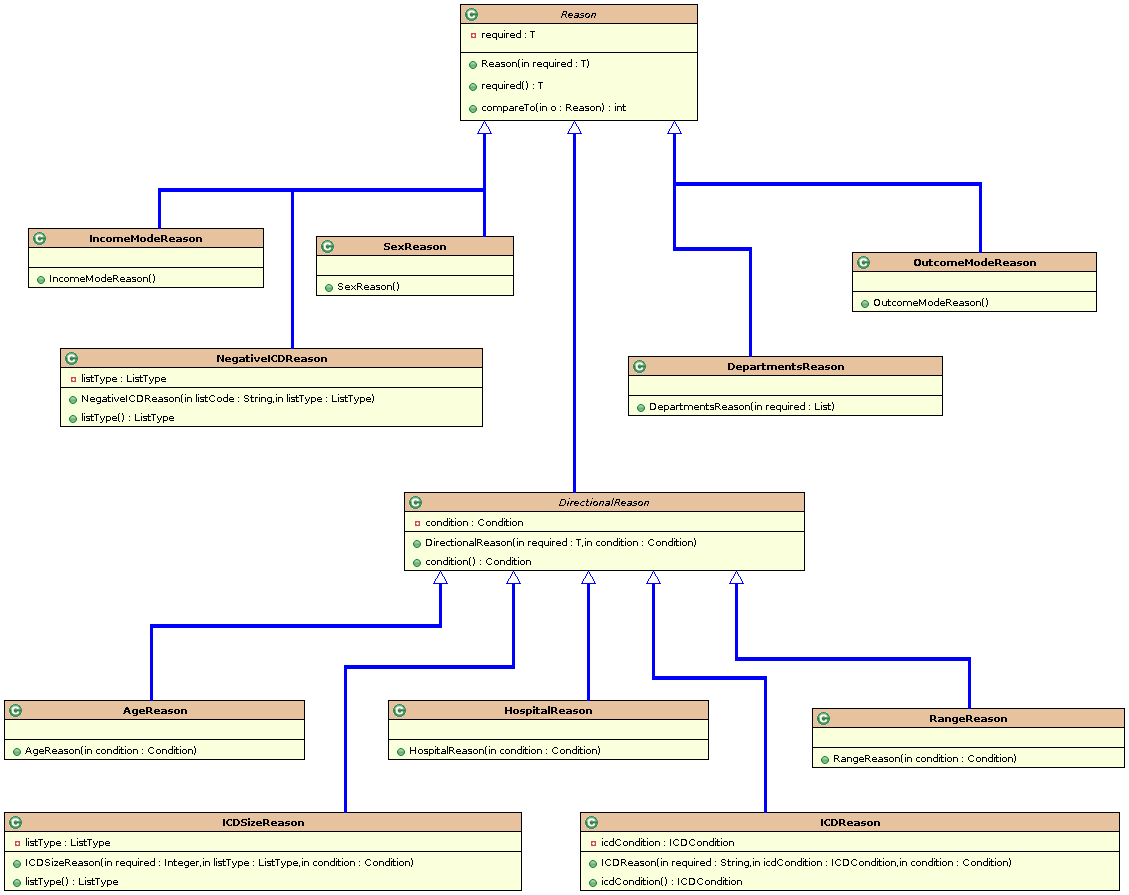
\includegraphics[scale=0.4]{images/reason-classes2}

Rozszerzyłem listę argumentów każdej z metod checkerów o argument: lista powodów niezaakceptowania: List<Reason> reasons. 
Po sprawdzeniu konkretnego warunku, w przypadku jego niezaakceptowania tworzona jest odpowiednia instancja obiektu Reason, a następnie jest ona  dodawana do listy. Np:
\begin{verbatim}
protected boolean checkHospitalLimit(Stay stay, HospitalLimit hospLimit, List<Reason> reasons) {
     if (hospLimit != null) {
         int time = stay.getEpisode().hospitalTime(hospLimit.getTimeUnit());
         boolean result = hospLimit.test(time);
         if (!result) {
             reasons.add(new HospitalReason(hospLimit, condition()));
         }
         return result;
     }
     return true;
}
\end{verbatim}

Np: Powodem niezaakceptowania grupy systemu JGP może być niespełnienie warunku: czas hospitalizacji dla grupy JGP musi być większy niż 7 dni, a zdefiniowany czas leczenia jest równy 5 dni.

Takie podejście pozwala na stworzenie funkocjonalności, która będzie podpowiadać lekarzowi jakie może uzyskać grupy JGP z większą wartości punktową, czyli jak zmaksymalizować koszty leczenia pacjenta. Program podpowiadałby również jakie konkretnie warunki musi spełnić hospitalizacja, aby zaliczyć ją do droższej grupy (wybranej przez lekarza).

Zaimplementowanie mechanizmu ,,Reasons - powody niezaakceptowania do grupy'' odpowiada w systemie ekspertowym modułowi objaśniająco-wyjąśniającemu(ang. Explanation Facility). Jest to część systemu odpowiedzialna za wyprowadzanie na zewnątrz wniosków systemu. Moduł ten daje użytkownikowi radę, sugestię, ale nie podejmuje decyzji. Zwróćmy uwagę, że zapis historii niespełnionych warunków pozwala odtworzyć część ścieżki poszukiwania rozwiązania dla rozwiązań niespełniających warunków.
